\section{Evaluation}
\label{sec:eval}

We ask five questions. Do the models agree with measured NASA data? Are search and selection correct? What does constraint-aware planning change? Does an independent implementation agree? Does the end-to-end system meet its budgets? \Cref{tab:evidence} summarizes the answers. We say a model \emph{reproduces} or is \emph{compared with} data; none of these checks validates the system for crewed use.

\begin{table*}[t]
  \centering\small
  \caption{Summary of the evidence. MAPE: mean absolute percentage error; MAE: mean absolute error; pp: percentage points. ``By construction'' means the property follows from the design and is checked by tests.}
  \label{tab:evidence}
  \begin{tabularx}{\textwidth}{@{}>{\raggedright\arraybackslash}p{0.26\textwidth} L L@{}}
    \toprule
    Check & Result & Main caveat \\
    \midrule
    Walking energy vs NASA suited data & MAPE 10.6\% at 0.22--0.32\,$g$ (17.6\% at our pace); 36.0\% at 0.12--0.17\,$g$ & Digitized trend lines; level walking under-predicted; 0.38\,$g$ extrapolated \\
    Terrain sky obstruction vs \citet{guo2026} & MAE 2.0\,pp, $r=0.94$ (15 periods) & Normalization chosen after seeing the data; one miss of 12\,pp \\
    Dose vs Curiosity RAD, year 1 & 198.8 vs 207.8\,µGy/day ($-4.3$\%) & $-8.7$\% at the scenario season; $-20$\% to $+41$\% over the solar cycle \\
    Leg search vs independent oracle & A$^\ast$ optimality gap 0.000\% (80 Gale cases) & One site, one seed \\
    Station selection vs brute force & Equal on 320 random instances & Up to seven stations \\
    Slope-masked routing & 75\% of routes contain a step over 20$^\circ$; 199 of 200 break a constraint & Naive baseline by design \\
    Science when time is short & $+5.0$\% (95\% CI 3.9--6.1\%) vs a checked greedy planner; never lower & Team science values \\
    Staging (Hab-1 vs PR-1) & Habitat infeasible under every single relaxation tested; rover feasible & One scenario habitat position \\
    Engine vs independent checker & Agree on 23 of 24 walks; the miss is a safe-side \nogo & 24 single-destination walks \\
    End-to-end system & Package 10,994\,B; visor link loss to autonomous 3.4\,s; re-plan 8.3\,ms median & One local run; no radio hardware \\
    \bottomrule
  \end{tabularx}
\end{table*}

\subsection{Physical models against measured data}
\label{sec:eval-models}

\begin{figure*}[t]
  \centering
  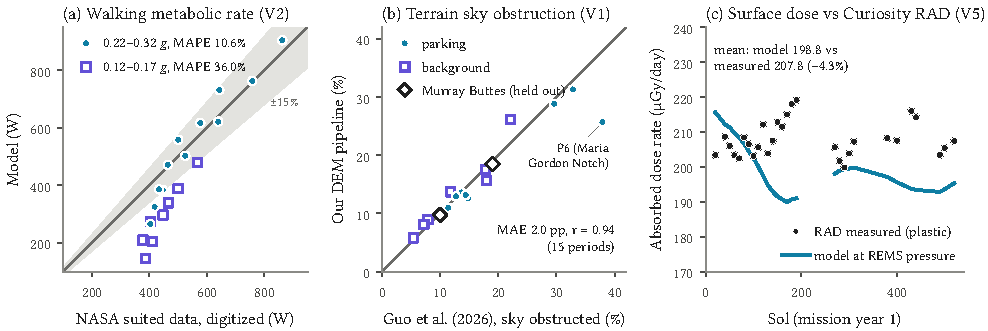
\includegraphics[width=0.92\textwidth]{eval_models.pdf}
  \caption{Model checks against measured NASA data. (a) Suited metabolic rate: model against NASA suited partial-gravity data \citep{norcross2010incline}, digitized from published trend lines (five gravity levels, four grades; band $\pm15$\%). (b) Terrain sky obstruction at Curiosity's parking positions and background periods against \citet{guo2026}; Murray Buttes was held out (reference value from \citealt{ehresmann2021}). (c) Daily absorbed dose in the RAD plastic detector over Curiosity's first Mars year against our model at measured REMS pressure.}
  \label{fig:models}
\end{figure*}

\paragraph{Walking energy.} NASA's Integrated Suit Test~2 measured six astronauts walking in a 121\,kg suit at 0.12--0.32\,$g$ on grades of 0--30\% \citep{norcross2010incline}. No table of means exists, so we digitized the per-gravity trend lines (point error about $\pm4$\% of power). We ran the model without fitting, using the subjects' mean mass of 80.7\,kg, no tools, $\eta=1$ and 0.765\,m/s, the midpoint of the reported speeds. At 0.22--0.32\,$g$ the MAPE is 10.6\%; at 0.56 and 0.97\,m/s, the ends of the speed range, it is 17.6\% and 18.7\%. At 0.12--0.17\,$g$ it is 36.0\% (\cref{fig:models}a). The model under-predicts level walking (by 34\% at 0.22\,$g$ and 62\% at 0.12\,$g$). The measured data show a floor of oxygen uptake that barely changes with gravity, whereas scaling the whole equation by $g$ drives the standing terms toward zero.

\paragraph{Terrain shielding.} \Citet{guo2026} tabulate the sky obstructed by terrain at Curiosity's parking positions and the resulting dose drops. Our pipeline casts rays from 1\,m above the DEM at Curiosity's waypoints. It reproduces the 15 obstruction values with an MAE of 2.0\,pp and $r=0.94$ (\cref{fig:models}b). We chose a solid-angle normalization after seeing the comparison; the two alternatives give 6.5 and 11.9\,pp. The largest miss, 12\,pp, is the narrow Maria Gordon notch. For held-out Murray Buttes we obtain 18.5\% obstruction against 19\% reported, but predict a dose drop of 8.4\% against a measured 4\%. Predicted drops have an RMSE of 4.3\,pp, against 5.1\,pp for always predicting the mean, so the shielding layer is labelled indicative.

\paragraph{Surface dose.} We compared the dose model with RAD daily dose \citep{hassler2012} on 29 first-year sols that have REMS pressure, excluding sols that a simple heuristic flags as affected by solar particle events. The measured mean is 207.8\,µGy/day and the model gives 198.8\,µGy/day ($-4.3$\%; \cref{fig:models}c). The first-year data imply $\Phi\approx518$\,MV rather than the assumed 600\,MV, which explains most of the bias. At the scenario season the model is 8.7\% low. Later years at the same season range from $-20$\% to $+41$\% of the first-year value, so route doses are indicative to a few tens of percent.

\subsection{Correctness of search and selection}
\label{sec:eval-planner}
A benchmark runs each search and cost model over 40 static and 40 hidden-hazard scenarios on the Gale grid. It scores paths against an independently written Dijkstra oracle (\cref{tab:bench} in \cref{app:tables}). A$^\ast$ is exactly optimal and expands about a quarter as many nodes as the engine's Dijkstra, whose 0.036\% gap we attribute to decisecond quantization. A slope-weighted cost model typical of generic tools finds paths that look 5\% cheaper only by taking 140--166 steps over the 20$^\circ$ step limit. The station DP equals brute force on 320 instances, and the property test in \cref{sec:sim} found no unsafe plan. All 138 unit tests passed on 15 November 2026.

\subsection{What constraint-aware planning changes}
\label{sec:eval-impact}

\begin{figure*}[t]
  \centering
  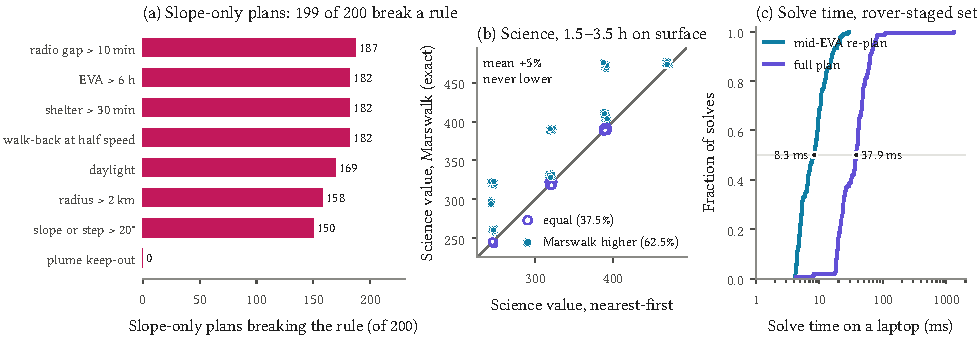
\includegraphics[width=0.92\textwidth]{eval_impact.pdf}
  \caption{Planning impact over simulated EVAs at Gale. (a) Slope-masked least-cost plans (200 rover-staged scenarios) that break each constraint when replayed in our simulator. (b) Science value of exact selection against a nearest-first planner with the same checks, with 1.5--3.5\,h of surface time (200 scenarios, jittered). (c) Solve times on a laptop.}
  \label{fig:impact}
\end{figure*}

We generated scenarios on the Gale pack with fixed seeds. The main set has 200 rover-staged EVAs requesting 3--6 of the 12 stations (60 more from the habitat). An oversubscribed set offers all 12 stations but leaves only 90--210\,min (1.5--3.5\,h) of surface time. \emph{Slope-masked} routing visits all requested stops along least-cost paths on a grid that blocks slopes over 20$^\circ$; it is naive by design. \emph{Nearest-first} adds the nearest stop only if the whole plan passes our checker; it is a greedy baseline with a perfect rule checker, which no human planner has.

Replayed in our simulator, 199 of 200 slope-masked plans break at least one constraint (\cref{fig:impact}a), mostly constraints that slope cannot see: radio gap (187), walk-back, shelter and EVA duration (182 each). Of the 200 routes, 150 (75\%) contain a step steeper than 20$^\circ$ between two cells that each pass the cell-slope mask. \Marswalk and nearest-first return no violating plan by construction; \cref{sec:eval-crosscheck} tests the checker independently. With a full EVA, the constraints are tight enough that nearest-first picks the same stations as \Marswalk in all 200 scenarios. When time is short, exact selection gains 5.0\% science value on average (paired bootstrap 95\% CI 3.9--6.1\%, median 1.1\%, maximum 30.6\%). It is better in 62.5\% of scenarios and never worse (\cref{fig:impact}b). Full plans take a median of 37.9\,ms and mid-EVA re-plans 8.3\,ms on a laptop (\cref{fig:impact}c), fast enough to re-plan on every telemetry update.

\subsection{Staging: habitat or rover}
\label{sec:eval-scenario}

\begin{figure*}[t]
  \centering
  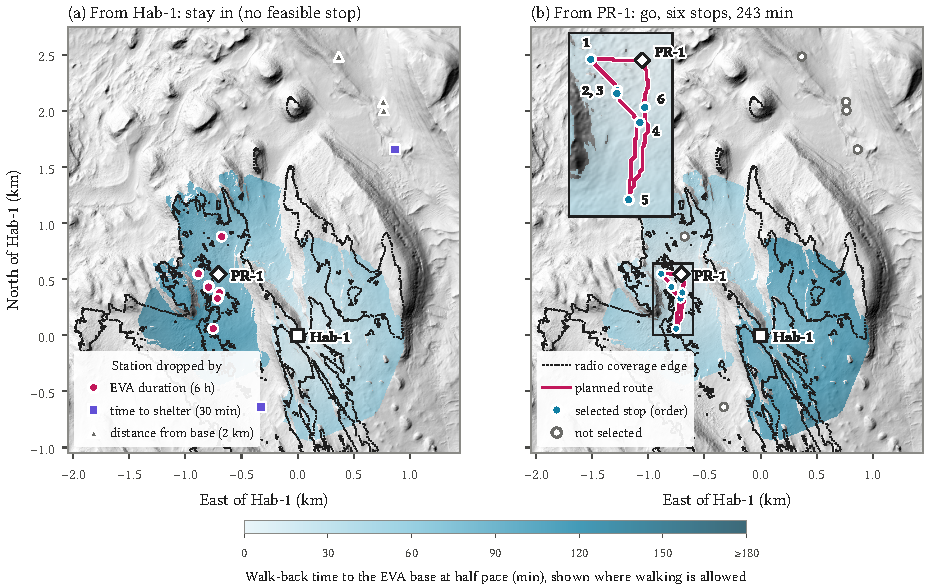
\includegraphics[width=0.78\textwidth]{scenario.pdf}
  \caption{The default scenario, planned by the engine. Shading: walk-back time to the EVA base where walking is allowed; dotted lines: edge of radio coverage. (a) From Hab-1 every station fails: seven exceed the 6-hour EVA once heat rests on the climb back are included, two exceed 30\,min to shelter and three lie beyond 2\,km. (b) From PR-1, a six-stop plan in 243\,min (inset: route and order; stops 2 and 3 are about 10\,m apart). The walkable footprint is the same from both bases. What differs is the time to get back: 80--115\,min from stations ST01--ST07 to Hab-1, against 8--30\,min to PR-1.}
  \label{fig:scenario}
\end{figure*}

The default scenario plans all twelve stations from the habitat at 09:40 LTST (\cref{fig:scenario}). The engine returns \stayin with EVA duration as the binding constraint, and adds that staging from the rover allows six stations. The seven boxwork stations lie 144--217\,m below the habitat and 0.75--1.1\,km away, so every walk to them ends in a loaded climb at 668--824\,W, roughly twice the heat budget. Staged from PR-1, the plan visits ST04, ST02, ST03, ST06, ST07 and ST05 for a science value of 475 in a 243-minute EVA (183\,min on the surface, including 9.5\,min of heat rests; \cref{fig:anatomy}). It never goes more than 487\,m from the rover, and its binding constraint is the radio gap, with a margin of 0.4\,min.

\begin{figure*}[t]
  \centering
  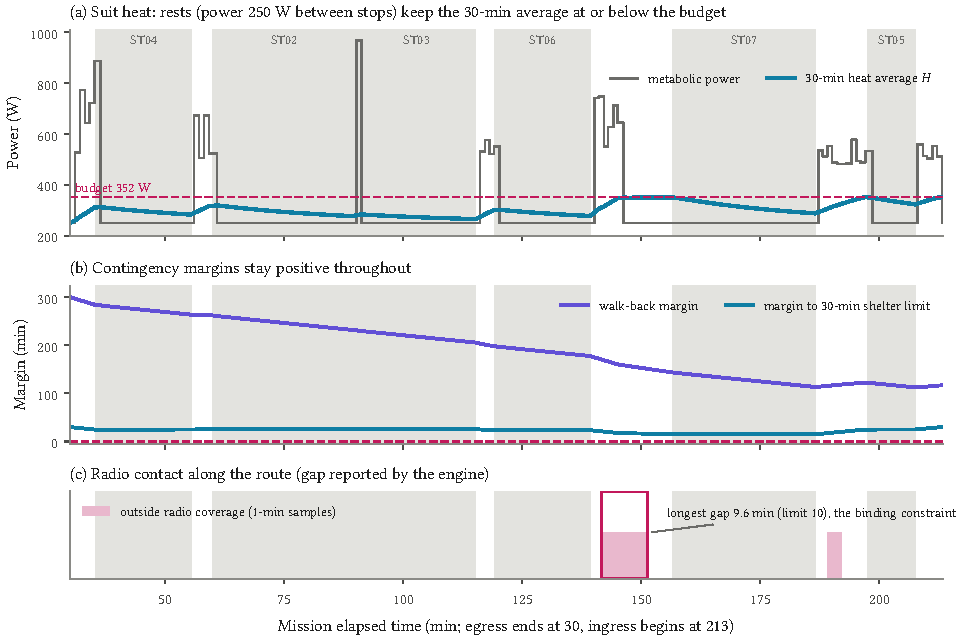
\includegraphics[width=0.72\textwidth]{anatomy.pdf}
  \caption{Anatomy of the six-stop plan from PR-1, from the engine's burndown (grey bands: stations). (a) Metabolic power and its 30-minute average against the 352\,W budget; rests at 250\,W between stops total 9.5\,min. (b) Walk-back margin and margin to the shelter limit. (c) Samples outside radio coverage; the engine's longest gap, 9.6\,min against a limit of 10, is the binding constraint.}
  \label{fig:anatomy}
\end{figure*}

\Cref{tab:sensitivity} varies one team-chosen parameter at a time. From the habitat, no single change makes any station walkable. Raising the heat budget to 530\,W, or removing it, turns the seven boxwork failures into radio-gap failures. Relaxing the radio gap alone leaves them failing on EVA duration. The walk-back pace, shelter limit and radius only change which of the other five stations fails first. Only lifting both the heat and radio-gap limits makes six stations walkable from the habitat. The boxwork stations are therefore blocked jointly by suit heat and radio contact, which a single-rule binding constraint cannot express. From the rover, the plan is robust to these parameters, and relaxing either heat or radio gap adds ST01 (value 555). Per-cell rules alone do not separate the two bases. From either base, the same 2.86\,km$^2$ and seven stations satisfy slope, keep-out, radius, shelter and out-and-back time (\cref{tab:ablation}). The difference arises only from constraints evaluated along the trajectory, which is why the simulator matters. This is our model's result for one habitat position, not a NASA finding. It agrees with DRA~5.0's use of pressurized rovers as mobile bases \citep{drake2009dra5} and shows that a crew-side planner can answer where to stage a walk, not only how to walk it.

\begin{table*}[t]
  \centering\small
  \caption{One-at-a-time sensitivity of the default scenario (all twelve stations, 09:40 LTST). Dropped: stations dropped per rule (EVA = duration, radio = radio gap, w-b = walk-back).}
  \label{tab:sensitivity}
  \begin{tabular}{@{}l l c c c l@{}}
    \toprule
    Base & Variant & Result & Stops & Value & Dropped \\
    \midrule
    Hab-1 & baseline & \stayin & 0 & -- & 7 EVA, 2 shelter, 3 radius \\
          & heat budget 530\,W, or heat limit off & \stayin & 0 & -- & 7 radio, 2 shelter, 3 radius \\
          & radio gap 20\,min, or radio-gap rule off & \stayin & 0 & -- & 7 EVA, 2 shelter, 3 radius \\
          & walk-back pace $0.67\times$ & \stayin & 0 & -- & 7 EVA, 2 shelter, 3 radius \\
          & shelter limit 45\,min & \stayin & 0 & -- & 7 EVA, 1 radio, 1 shelter, 3 radius \\
          & radius 3\,km & \stayin & 0 & -- & 7 EVA, 5 shelter \\
          & heat limit and radio-gap rule both off & \go & 6 & 470 & 1 w-b, 2 shelter, 3 radius \\
    \midrule
    PR-1  & baseline & \go & 6 & 475 & 1 radio, 2 shelter, 3 radius \\
          & heat budget 530\,W, or heat limit off & \go & 7 & 555 & 2 shelter, 3 radius \\
          & radio gap 20\,min, or radio-gap rule off & \go & 7 & 555 & 2 shelter, 3 radius \\
          & walk-back pace, shelter limit or radius (as above) & \go & 6 & 475 & radius and shelter drops shift \\
    \bottomrule
  \end{tabular}
\end{table*}

\subsection{Independent cross-check}
\label{sec:eval-crosscheck}
We sampled 24 single-destination walks at Gale: 12 \go and 12 \nogo, with the \nogo cases spread across the failing rules. An independently written Python checker decodes the site pack itself and recomputes slope, step grades, line of sight (with curvature), keep-outs, sun elevation, walk-back and shelter times. It shares only route cells, rule values, mast positions and rasters with the engine, and it omits the heat governor. Engine and checker agree on 23 of 24 walks, and on all 96 rule-level checks that do not depend on heat rests (no walk fails slope or keep-out, so only radius and shelter discriminate). In the one disagreement, the engine called a walk \nogo because its heat-aware route spent 0.22\,min too long out of contact. The shortest-time path stays within the limit, and the engine's own simulator confirms it passes, but the planner did not try it. The error is on the safe side. Two blind AI judges, given the rules and engine-generated evidence, matched the same 23 verdicts. They test rule application only, and they share a model family with the agents that wrote much of the code.

\subsection{End-to-end system}
\label{sec:eval-system}
An automated test runs the habitat server, console and visor as three local processes with the real engine and the Gale pack (one run). The phone navigator reuses the visor's controller but is not part of this test, so these figures are for the visor. The first plan solves cold in 1.6\,s. The signed 10,994-byte package is verified on the visor 168\,ms after ``Send to crew''. A simulated radiation spike produces a return route in 2\,ms (668\,ms to the screen). After a link drop the visor becomes autonomous in 3.4\,s, and queued telemetry back-fills within 1.8\,s of recovery. These timings come from a local network, not from radio hardware.
